% Solution for Problem 031
% Source: 38회(2024) KMO 중등부 1차 20번
% Original file: Problem Sets/contents/quiz05.tex


\fbox{ 38회(2024) KMO 중등부 1차 20번 }\\
답 : 512
%\import{images}{38_20}

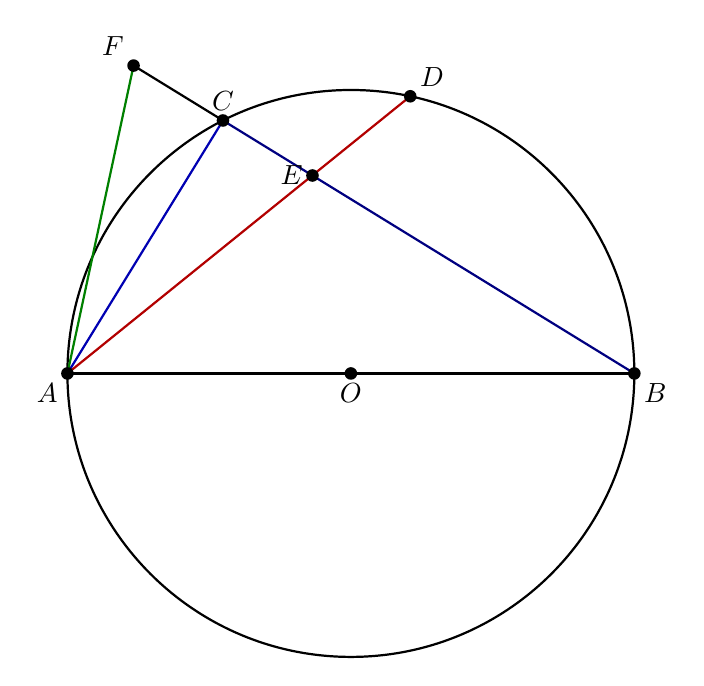
\begin{tikzpicture}[scale=0.2]
    % Step 1: 좌표 정의
    \coordinate (O) at (0,0);
    \coordinate (A) at (-18,0);
    \coordinate (B) at (18,0);

    % Step 2: 점 C 계산
    % 원 위의 점, B로부터 거리 = 24 + 20/3 = 92/3
    % Cx = (648 - (92/3)^2) / 36 ≈ -8.123
    % Cy = sqrt(324 - Cx^2) ≈ 16.063
    \coordinate (C) at (-8.123, 16.063);

    % Step 3: 점 D 계산
    % C의 각도 ≈ 116.86° → D의 각도 ≈ 77.91°
    \coordinate (D) at (3.77, 17.60);

    % Step 4: 점 E 계산 (AD와 BC의 교점)
    % t = 0.7144, E = A + t(D-A)
    \coordinate (E) at (-2.44, 12.57);

    % Step 5: 점 F 계산 (BC 연장선 위, CF = CE)
    % CE ≈ 6.67, BC 방향으로 C에서 연장
    \coordinate (F) at (-13.80, 19.55);

    % 원 O (AB를 지름으로 함)
    \draw[thick] (O) circle (18);

    % Step 1: 선분 AB (지름)
    \draw[thick] (A) -- (B);

    % Step 2: 선분 AC, BC
    \draw[thick, blue!70!black] (A) -- (C);
    \draw[thick, blue!50!black] (B) -- (C);

    % Step 4: 선분 AD
    \draw[thick, red!70!black] (A) -- (D);

    % Step 5: 선분 AF
    \draw[thick, green!50!black] (A) -- (F);

    % 점 표시
    \foreach \point/\position in {O/below, A/below left, B/below right, C/above, D/above right, E/left, F/above left} {
        \fill (\point) circle (0.4);
        \node[\position] at (\point) {$\point$};
    }

    \draw[thick] (C) -- (F);

\end{tikzpicture}

선분 $BC$ 의 $C$ 쪽으로의 연장선 위에 $\overline{CE} = \overline{CF}$ 를 만족하는 점 $F$ 을 찾는다. \\
$\angle ACB $ 가 직각이므로 $\overline{AF} = \overline{AE} = 20$ 이다. \\
이제 직선 $AD$ 는 삼각형 $ABF$ 에서 각 $A$ 의 이등분선이므로 이등분선의 성질을 이용할 수 있다. 
\[ \overline{AF} : \overline{AB} = \overline{EF} : \overline{BE} \]
$ \overline{CE} = \overline{CF} = 5k $ ,  $\overline{BE} = 18k$ 로 하고 $\overline{AC} = h$ 로 두자. \\
두 직각삼각형에 피타고라스 정리를 적용 두 개의 식을 얻고 $k$의 값을 구할 수 있다.
